% !TeX spellcheck = en_GB
% !TeX program = pdflatex
%
% LuxSleek-CV 1.1 LaTeX template
% Author: Andreï V. Kostyrka, University of Luxembourg
%
% 1.1: added tracking and letter-spacing for prettier lower caps, added `~` for language levels
% 1.0: initial release
%
% This template fills the gap in the available variety of templates
% by proposing something that is not a custom class, not using any
% hard-coded settings deeply hidden in style files, and provides
% a handful of custom command definitions that are as transparent as it gets.
% Developed at the University of Luxembourg.
%
% *NOTHING IS HARCODED, and never should be.*
%
% Target audience: applicants in the IT industry, or business in general
%
% The main strength of this template is, it explicitly showcases how
% to break the flow of text to achieve the most flexible right alignment
% of dates for multiple configurations.

\documentclass[11pt, a4paper]{article} 


\usepackage[T1]{fontenc}     % We are using pdfLaTeX,
\usepackage[utf8]{inputenc}  % hence this preparation
\usepackage[british]{babel}  
\usepackage[left = 0mm, right = 0mm, top = 0mm, bottom = 0mm]{geometry}
\usepackage[stretch = 25, shrink = 25, tracking=true, letterspace=30]{microtype}  
\usepackage{graphicx}        % To insert pictures
\usepackage{xcolor}          % To add colour to the document
\usepackage{marvosym}        % Provides icons for the contact details
\usepackage{fontawesome}
\usepackage{setspace}
\usepackage{enumitem}        % To redefine spacing in lists
\setlist{parsep = 0pt, topsep = 0pt, partopsep = 1pt, itemsep = 1pt, leftmargin = 6mm}

\usepackage{FiraSans}        % Change this to use any font, but keep it simple
\renewcommand{\familydefault}{\sfdefault}

\definecolor{cvblue}{HTML}{304263}

%%%%%%% USER COMMAND DEFINITIONS %%%%%%%%%%%%%%%%%%%%%%%%%%%
% These are the real workhorses of this template
\newcommand{\dates}[1]{\hfill\mbox{\textbf{#1}}} % Bold stuff that doesn’t got broken into lines
\newcommand{\is}{\par\vskip.5ex plus .4ex} % Item spacing
\newcommand{\smaller}[1]{{\small$\diamond$\ #1}}
\newcommand{\headleft}[1]{\vspace*{3ex}\textsc{\textbf{#1}}\par%
    \vspace*{-1.5ex}\hrulefill\par\vspace*{0.7ex}}
\newcommand{\headright}[1]{\vspace*{2.5ex}\textsc{\Large\color{cvblue}#1}\par%
     \vspace*{-2ex}{\color{cvblue}\hrulefill}\par}
%%%%%%%%%%%%%%%%%%%%%%%%%%%%%%%%%%%%%%%%%%%%%%%%%%%%%%%%%%%%
\usepackage{fontawesome}
\usepackage[colorlinks = true, urlcolor = magenta, linkcolor = white]{hyperref}

\begin{document}

% Style definitions -- killing the unnecessary space and adding the skips explicitly
\setlength{\topskip}{0pt}
\setlength{\parindent}{0pt}
\setlength{\parskip}{0pt}
\setlength{\fboxsep}{0pt}
\pagestyle{empty}
\raggedbottom

\begin{minipage}[t]{0.33\textwidth} %% Left column -- outer definition
%  Left column -- top dark rectangle
\colorbox{pink}{\begin{minipage}[t][5mm][t]{\textwidth}\null\hfill\null\end{minipage}}

\vspace{-.2ex} % Eliminates the small gap
\colorbox{pink!60}{\color{black}  %% LEFT BOX
\kern0.09\textwidth\relax% Left margin provided explicitly
\begin{minipage}[t][293mm][t]{0.82\textwidth}
\raggedright
\vspace*{2.5ex}

\Large Vajihe \textbf{\textsc{Mobasheri}} \normalsize 

% Centering without extra vertical spacing
\null\hfill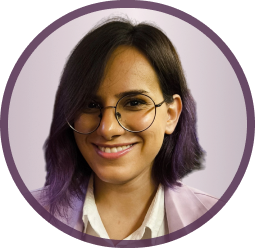
\includegraphics[width=0.65\textwidth]{photo.png}\hfill\null

\vspace*{0.5ex} % Extra space after the picture

\headleft{Profile}
I'm a Data Science graduate with a keen interest in the application of Artificial Intelligence in the medical field. My master's thesis focused on disease diagnosis using medical images, where I developed deep learning models to improve diagnostic accuracy. I also have work experience in Business Intelligence and Artificial Intelligence. I'm eager to pursue a Ph.D. in AI, focusing on its applications in healthcare, to contribute to innovative research that integrates data science with medical advancements.
% I am a Data Science graduate with experience in disease diagnosis using medical images for my master's thesis. I have also worked in Business Intelligence and Artificial Intelligence, enhancing my analytical skills. I am eager to pursue a Ph.D. in AI, focusing on its applications in healthcare, to contribute to innovative research that integrates data science with medical advancements.
%image processing must be adde.
% medical image must be added.


\headleft{Contact details}
\small % To fit more content
\faEnvelopeO\  \href{mailto:vajihemobasheri76@gmail.com}{vajihemobasheri76@gmail.com} \\[0.1ex]
\faPhone\ +98\,921\,875\,95\, 29 \\[0.5ex]
\faGlobe\ \href{https://vajihemobasheri76.wixstudio.io/mycv}{vajihemobasheri76.wixstudio.io} \\[0.1ex]
\faGithub\ \href{https://github.com/VajiheMobasheri}{github.com/VajiheMobasheri} \\[0.1ex]
\faLinkedinSquare\ \href{https://www.linkedin.com/in/vajihe-mobasheri-a2b796231}{linkedin.com/in/VajiheMobasheri} \\[0.1ex]
\faLocationArrow\ Tehran, Iran
\normalsize

\headleft{Personal information}
Date of birth: \textbf{13/03/1998} \\[0.5ex]
Citizenship: \textbf{Iran} \\[0.5ex]
Family: \textbf{Single} \\[0.5ex]
Languages: \textbf{English}~(B2), \textbf{Persian}~(native)


\headleft{Soft Skills}
\begin{itemize}
\item Teamwork
\item Responsible
%\item Fast learn
%\item Analytical thinking 
%\item Flexibility 
\item Crisis Management
\item Good interpersonal skills
%\item Active listening 
\end{itemize} 


\headleft{Hobbies}
\begin{itemize}
\item Reading (psychology and Personal Development)
% \item Cooking
\item Gardening 
\end{itemize} 




\end{minipage}%
\kern0.09\textwidth\relax%%Right margin provided explicitly to stretch the colourbox
}
\end{minipage}% Right column
\hskip2.5em% Left margin for the white area
\begin{minipage}[t]{0.56\textwidth}
\setlength{\parskip}{0.8ex}% Adds spaces between paragraphs; use \\ to add new lines without this space. Shrink this amount to fit more data vertically

\vspace{2ex}
\headright{Research Interest}
\smaller{Image Processing} \smaller{Deep Learning} \smaller{Computer Vision} \smaller{Artificial Intelligence}


\headright{Education}
\textsc{Master in Data Sciense(supervised by Dr. Sohrab Effati)}.Faculty of Mathematics. \textit{Ferdowsi University of Mashhad}. \dates{2022--2024} \\
\smaller{Thesis title: \textit{Classification of medical images containing noise using least squares twin support vector machine method
with uncertain data.}} \\
\smaller{Classification, Image Processing.}\\
\smaller{Grade: 3.68/4}\\
\is
\textsc{Bachelor of Applied Mathematics.} Faculty of Mathematics. \textit{Ferdowsi University of Mashhad}.  \dates{2016--2021} 


\headright{Work Experience}
\textsc{AI Researcher} at \textit{Faraz Pajohan.}  \dates{2024.03--pres.} \\
\smaller{Conducting research on large language models and artificial intelligence to identify optimal methods and tools for product development.}\\
\smaller{Utilizing frameworks like LangChain and ChainLit for AI-driven solutions.}\\
\smaller{Writing research articles to support product ideas and innovations.}\\
\is % Item spacing -- defined in the preamble
\textsc{Business Intelligence Analyst } at \textit{Faraz Pajohan.}  \dates{2022.10--2024.3} \\
\smaller{Data Analysis.}\\
\smaller{Designing KPI Dashboards and Data Visualization.}


\headright{Skills}
\is
\textit{Programming Languages:} \texttt{Python}
\is
\textit{Libraries:} \texttt{Pandas, Numpy, Sk-learn, Vega-Altair, Matplotlib}
\is
\textit{AI Frameworks:} \texttt{LangChain, ChainLit, Dify}
\is
\textit{Relational Databases:} \texttt{MySQL}
\is
\textit{NoSQL Databases:} \texttt{Elasticsearch}
\is
\textit{Tools:} \texttt{Git, PowerBI, Tableau, \LaTeX}


\headright{Projects}
\textsc{Danayar}\\
\smaller{Developed an AI system called "Danayar" that processes organizational documents and enables a question-answering interface with document referencing at \textit{Faraz Pajohan.}}\dates{2024}\\
\smaller{Technologies Used: \texttt{LangChain, Chainlit, Retrieval-Augmented Generation(RAG)}}


\headright{Presentation}
\textit{What is Gradient Descent?} \dates{2024}\\
\textit{Attention Is All You Need.} \dates{2023}\\
\textit{What is Elasticsearch?} \dates{2023}\\
\textit{What is Feature Selection?} \dates{2022}\\
\textit{What is PCA and how does it work?} \dates{2022}

\end{minipage}

\newpage
\hskip2.5em% Left margin for the white area
\begin{minipage}[t]{0.90\textwidth}
\setlength{\parskip}{0.8ex}% Adds spaces between paragraphs; use \\ to add new lines without this space. Shrink this amount to fit more data vertically

\vspace{2ex}
\headright{Selected Cources}
\begin{tabular}{l @{\hspace{4cm}} c @{\hspace{1cm}} l @{\hspace{2cm}} c}
\smaller{Big Data} & 3.6/4 & \smaller{Optimization and Neural Networks} & 3.4/4 \\
\smaller{Text Mining} & 3.5/4 & \smaller{Mathematical Foundations of Data Science} & 3.4/4 \\
\smaller{Machine Learning} & 3.4/4 & \smaller{Data Science Algorithms} & 3.4/4 \\
\end{tabular}


\headright{Publications}
\textit{Danayar: A Secure and Intelligent Companion for Organizational Managers in Data-Driven Analysis and Decision-Making.}\dates{2024}\\
\smaller{\textcolor{magenta}{Vajihe Mobasheri}; Rasoul Ramezanian; MuhammadReza FatehiNia; Somaye Soltani}\\
\smaller{Type: \textit{Academic-Industrial Research Paper}}\\
\smaller{21\textsuperscript{th} International Conference of the Iranian Society of Cryptology.}


\headright{Certificates}
\textsc{Comprehensive Data Science Specialization} \dates{2021--2022}\\
\smaller{}\href{https://ut.ac.ir/en}{Tehran University}
\is
\textsc{Dashboard design with Microsoft Power BI} \dates{2021}\\
\smaller{}\href{https://mftplus.com/}{Tehran Institute of Technology}


\headright{Other Activities}
\textsc{Organizer of 3 Power BI Training Workshops.}Faculty of Mathematics.\\ \textit{Ferdowsi University of Mashhad}. \dates{2021,2022,2024}\\
\smaller{Scientific Association of Statistics.}


\headright{References}
	{\textbf{\href{https://scholar.google.com/citations?hl=en&user=g0onknYAAAAJ}{Prof. Sohrab Effati}}}\\
	\textsc{Position:}{Professor}{}\\
	\textsc{Employer:}{Ferdowsi University of Mashhad, Iran}{}\\
	\textsc{Email:}\href{mailto:s-effati@um.ac.ir}{s-effati@um.ac.ir}
    \is
	{\textbf{\href{https://scholar.google.com/citations?user=9kzGRJgAAAAJ&hl=en}{Prof. Omid Soleimani-Frad}}}\\
	\textsc{Position:}{Associate Professor}{}\\
	\textsc{Employer:}{Ferdowsi University of Mashhad, Iran}{}\\
	\textsc{Email:}\href{mailto:soleimani@um.ac.ir}{soleimani@um.ac.ir},\href{mailto:omidsfard@gmail.com}{omidsfard@gmail.com}
    \is
	{\textbf{\href{https://scholar.google.com/citations?user=edYFIQEAAAAJ&hl=en}{Prof. Rasoul Ramezanian}}}\\
	\textsc{Position:}{Senior Researcher}{}\\
	\textsc{Employer:}{University of Lausanne, HEC, Switzerland}{}\\
	\textsc{Email:}\href{mailto:rasoul.ramezanian@unil.ch}{rasoul.ramezanian@unil.ch},\href{mailto:rasool.ramezanian@gmail.com}{rasool.ramezanian@gmail.com}
\end{minipage}






%personal site
%Grade,rank
\end{document}
